\documentclass[10pt,a4paper,twocolumn,twoside]{article}
\usepackage[utf8]{inputenc}
\usepackage[catalan]{babel}
\usepackage{multicol}
\usepackage{graphicx}
\usepackage{fancyhdr}
\usepackage{times}
\usepackage{titlesec}
\usepackage{multirow}
\usepackage{lettrine}
\usepackage[top=2cm, bottom=1.5cm, left=2cm, right=2cm]{geometry}
\usepackage[figurename=Fig.,tablename=TAULA]{caption}
\captionsetup[table]{textfont=sc}
% \usepackage{urlbst}



\author{\LARGE\sffamily Pol Colomer Campoy}
\title{\Huge{\sffamily Desenvolupament d'una Plataforma per a l'Anàlisi i Generació de Partitures Musicals a partir d'Àudio Multitrack}}


\newcommand\blfootnote[1]{%
  \begingroup
  \renewcommand\thefootnote{}\footnote{#1}%
  \addtocounter{footnote}{-1}%
  \endgroup
}

%
%\large\bfseries\sffamily
\titleformat{\section}
{\large\sffamily\scshape\bfseries}
{\textbf{\thesection}}{1em}{}

\begin{document}

\fancyhead[LO]{\scriptsize AUTOR: TÍTOL DEL TREBALL}
\fancyhead[RO]{\thepage}
\fancyhead[LE]{\thepage}
\fancyhead[RE]{\scriptsize EE/UAB TFG INFORMÀTICA: TÍTOL (ABREUJAT SI ÉS MOLT LLARG)}

\fancyfoot[CO,CE]{}

\fancypagestyle{primerapagina}
{
   \fancyhf{}
   \fancyhead[L]{\scriptsize TFG EN ENGINYERIA INFORMÀTICA, ESCOLA D'ENGINYERIA (EE), UNIVERSITAT AUTÒNOMA DE BARCELONA (UAB)}
   \fancyfoot[C]{\scriptsize ``Mes'' de 20xx, Escola d'Enginyeria (UAB)}
}

%\lhead{\thepage}
%\chead{}
%\rhead{\tiny EE/UAB TFG INFORMÀTICA: TÍTOL (ABREUJAT SI ÉS MOLT LLARG)}
%\lhead{ EE/UAB \thepage}
%\lfoot{}
%\cfoot{\tiny{Mes 2024, Escola d'Enginyeria (UAB)}}
%\rfoot{}
\renewcommand{\headrulewidth}{0pt}
\renewcommand{\footrulewidth}{0pt}
\pagestyle{fancy}

%\thispagestyle{myheadings}
\twocolumn[\begin{@twocolumnfalse}

%\vspace*{-1cm}{\scriptsize TFG EN ENGINYERIA INFORMÀTICA, ESCOLA D'ENGINYERIA (EE), UNIVERSITAT AUTÒNOMA DE BARCELONA (UAB)}

\maketitle

\thispagestyle{primerapagina}
%\twocolumn[\begin{@twocolumnfalse}
%\maketitle
%\begin{abstract}
\begin{center}
\parbox{0.915\textwidth}
{\sffamily
\textbf{Resum--}
TODO: Aconseguir separar pistes d’àudio donat un àudio multitrack i obtenir les notes de cada pista per posteriorment generar la partitura de la mateixa. Estudiar els resultats obtinguts per diferents algoritmes amb diferents configuracions i combinacions d’àudios.
\\
\\
\textbf{Paraules clau-- } Paraules clau del treball, màxim 2 línies . .... ........ ........... .......... ..  TODO Multitrack, .\\
\\
%\end{abstract}
%\bigskip
%\begin{abstract}
\bigskip
\\
\textbf{Abstract--} 
TODO: To separate audio tracks by giving a multitrack audio and obtain the notes of each track to later generate the score of it. Study the results obtained by different algorithms with different configurations and audio combinations.
\\
\\
\textbf{Keywords-- } Versió en anglès de les paraules clau. .... ........ ........... .......... ..  ... ..... .... ........ ........... .......... ..  ... ..... .... ........ ........... .................. ..\\
}

\bigskip

{\vrule depth 0pt height 0.5pt width 4cm\hspace{7.5pt}%
\raisebox{-3.5pt}{\fontfamily{pzd}\fontencoding{U}\fontseries{m}\fontshape{n}\fontsize{11}{12}\selectfont\char70}%
\hspace{7.5pt}\vrule depth 0pt height 0.5pt width 4cm\relax}

\end{center}

\bigskip
%\end{abstract}
\end{@twocolumnfalse}]

\blfootnote{$\bullet$ E-mail de contacte: Pol.ColomerC@autonoma.cat}
\blfootnote{$\bullet$ Menció realitzada: Computació}
\blfootnote{$\bullet$ Treball tutoritzat per: Felipe Lumbreras (departament - CVC)}
\blfootnote{$\bullet$ Curs 2023/2024}

\textbf{Resum--}
TODO: Aconseguir separar pistes d’àudio donat un àudio multitrack i obtenir les notes de cada pista per posteriorment generar la partitura de la mateixa. Estudiar els resultats obtinguts per diferents algoritmes amb diferents configuracions i combinacions d’àudios.


\section{Introducció - Context del treball}
\label{sec:intro}

\lettrine[lines=3]{E}{n} els darrers anys, el camp de l'enginyeria informàtica ha experimentat un notable avanç en el tractament del senyal d'àudio i en l'anàlisi musical automatitzada. El meu projecte d'enginyeria informàtica, que implica la separació d'instruments, la generació de partitures i la creació de tutorials visuals, s'ubica en la intersecció de diverses àrees de recerca i desenvolupament. La meva principal motivació és adquirir pràctica, comprensió i realitzar una investigació en l'àmbit de l'àudio, ja que durant la meva carrera, és un dels temes que han quedat menys explorats. D'aquesta manera, pretenc enriquir la meva experiència com a estudiant en aquest àmbit.


\section{Objectius}
\label{sec:objectius}

L'objectiu principal d'aquest projecte és aconseguir la separació de pistes d'àudio d'un arxiu multitrack i obtenir les notes musicals de cada pista per a la posterior generació de la seva partitura. A continuació, es detallen els objectius ramificats en forma d'arbre:

\begin{enumerate}
    \item Recopilar i preparar les dades necessàries per al desenvolupament del projecte, incloent-hi toy problems, arxius MIDI i àudios de concerts.
    \begin{enumerate}
        \item Elaborar i preparar toy problems representatius dels casos d'ús.
        \item Recopilar arxius MIDI de cançons amb els seus respectius ground truths.
        \item Obtenir àudios multitrack de concerts amb soroll ambient del públic per a casos més desafiant.
    \end{enumerate}
    \item Desenvolupar algoritmes i tècniques per a la separació de pistes d'àudio tant amb tècniques clàssiques com actuals 
    \begin{enumerate}
        \item Investigar i seleccionar algoritmes clàssics com Independent Component Analysis (ICA), Principal Component Analysis (PCA), Non-negative Matrix Factorization (NMF) i algorismes de filtratge per a la separació de pistes.
        \item Explorar les possibilitats de les tècniques de Deep Learning com Xarxes Neuronals Convolucionals (CNNs), Xarxes Neuronals Recurrents (RNNs), U-Net, Wave-U-Net i Deep Clustering per millorar la separació de pistes.
    \end{enumerate}
    \item Obtindre les notes musicals de cada pista separada:
    \begin{enumerate}
        \item Desenvolupar mètodes d'extracció de característiques i anàlisi musical per obtenir les notes musicals de cada pista separada.
    \end{enumerate}
    \item Generar la partitura musical de cada pista:
    \begin{enumerate}
        \item Implementar algoritmes per a la generació de partitures utilitzant la informació de les notes musicals obtingudes.
    \end{enumerate}
\end{enumerate}

\section{Tasques}
\label{sec:tasques}

Per assolir els objectius establerts, s'han definit les següents tasques, les quals estan dissenyades per abordar de manera efectiva els diversos aspectes del projecte:

\begin{enumerate}
    \item Recopilació de dades i preparació: (5 setmanes en total (paral·lel)
    \begin{enumerate}
        \item Investigar i seleccionar una varietat de toy problems representatius dels casos d'ús. (1 setmana)
        \item Recopilar una col·lecció d'arxius MIDI de diverses cançons juntament amb les seves partitures corresponents. (1 setmana)
        \item Obtindre àudios multitrack de concerts amb soroll ambient del públic per a casos més desafiant i variats. (1 setmana)
        \item Pre-processar i netejar les dades recopilades per garantir la seva qualitat i coherència. (2 setmanes)
    \end{enumerate}
    
    \item Desenvolupament d'algoritmes i tècniques per a la separació de pistes d'àudio:
    \begin{enumerate}
        \item Realitzar una revisió exhaustiva per identificar i comprendre els algoritmes clàssics i tècniques de Deep Learning més adequats per a la separació de pistes d'àudio. (2 setmanes)
        \item Implementar una gamma d'algoritmes clàssics com ara Independent Component Analysis (ICA), Principal Component Analysis (PCA), Non-negative Matrix Factorization (NMF) i algorismes de filtratge per explorar la seva eficàcia en la separació de pistes. (3 setmanes)
        \item Investigar i experimentar amb les tècniques de deep learning, incloent-hi Xarxes Neuronals Convolucionals (CNNs), Xarxes Neuronals Recurrents (RNNs), U-Net, Wave-U-Net i Deep Clustering, per millorar la qualitat i la precisió de la separació de pistes. (4 setmanes)
        \item Avaluar i comparar el rendiment dels diferents algoritmes i tècniques implementades utilitzant mètriques rellevants com la relació senyal-soroll (SNR), la separació de font de bescanvi (SiSdr) i la puntuació de seguiment de referència (SAR). (2 setmanes)
    \end{enumerate}
    
    \item Obtenció de les notes musicals de cada pista separada:
    \begin{enumerate}
        \item Investigar i desenvolupar mètodes d'extracció de característiques i anàlisi musical per obtenir les notes musicals de cada pista separada. (1 setmana)
        \item Implementar algoritmes d'anàlisi de freqüències, reconeixement de patrons i sincronització temporal per a l'extracció precisa de les notes musicals. (3 setmanes)
        \item Provar i ajustar els mètodes d'extracció de notes en diferents escenaris i tipus de pistes d'àudio. (1 setmana)
    \end{enumerate}
    
    \item Generació de partitures:
    \begin{enumerate}
        \item Desenvolupar algoritmes i processos per a la generació automàtica de partitures a partir de les notes musicals obtingudes. (3 setmanes)
        \item Implementar funcionalitats addicionals com la detecció de claus i la transcripció automàtica de les partitures generades. (2 setmanes)
        \item Validar les partitures generades mitjançant comparació amb les partitures originals i avaluació manual de la seva qualitat musical. (1 setmana)
    \end{enumerate}
    \item Documentació del projecte:
    \begin{enumerate}
        \item Preparar un Jupyter Notebook exhaustiu que descriu el procés complet del projecte, des de la recopilació de dades fins a la generació de partitures, incloent-hi explicacions detallades, codi font i visualitzacions. (2 setmanes)
        \item Crear una documentació detallada que explica els passos realitzats, els resultats obtinguts, les conclusions del projecte i les possibilitats de desenvolupament futur. (3 setmanes)
        \item Preparar una presentació o demostració del projecte per a l'avaluació final, incloent-hi la mostra dels resultats, les comparacions i les explicacions pertinents. (2 setmanes)
        \item Documentar i elaborar els informes per a cada entrega (2 setmanes)
    \end{enumerate}
\end{enumerate}

\section{Estat de l'Art}
\label{sec:estat_art}

En aquesta secció, intentaré fer un resum dels treballs rellevants en el camp de la separació de pistes d'àudio i la generació de partitures automàtiques.

La separació de pistes d'àudio és un tema amplament investigat en l'àmbit de la processament de senyals i la música computacional. En l'actualitat, s'han desenvolupat diverses tècniques per aconseguir aquest objectiu, que van des de mètodes clàssics fins a enfocaments basats en Deep Learning.

Entre els mètodes clàssics més utilitzats es troben l'Independent Component Analysis (ICA) \cite{ICA_Sawada_Ono_Kameoka_Kitamura_Saruwatari_2019}, que intenta descompondre l'àudio en fonts independents \cite{ICA_hyvarinen2000independent}, la Principal Component Analysis (PCA), que cerca les components principals de l'àudio \cite{PCA_jolliffe2002principal}, i la Non-negative Matrix Factorization (NMF), que divideix l'àudio en components no negatives \cite{NMF_lee1999learning}. Aquests mètodes han demostrat ser eficaços en diverses tasques de separació de pistes d'àudio, tot i que poden tenir limitacions en situacions de senyals molt complexes.

D'altra banda, els mètodes basats en Deep Learning han guanyat popularitat en els últims anys, especialment amb l'aparició de xarxes neuronals profundes. Les Xarxes Neuronals Convolucionals (CNNs), les Xarxes Neuronals Recurrents (RNNs) i les arquitectures especialitzades com la U-Net i la Wave-U-Net han estat utilitzades amb èxit per a tasques de separació de pistes d'àudio \cite{hershey2016deep,grill2017two,CNN_jansson2017singing,lva2018waveunet}. Aquests models són capaços d'aprendre representacions de nivell alt i baix de l'àudio, permetent una millor separació de les pistes.

Pel que fa a la generació de partitures automàtiques, s'han desenvolupat diversos mètodes per convertir les dades d'àudio en notació musical. Aquests mètodes inclouen la detecció de notes \cite{raffel2014mir_eval}, l'anàlisi harmònica \cite{pardo2002improved}, el reconeixement de melodies \cite{abdallah2004fundamental}, i la transcripció automàtica \cite{benetos2013automatic}. Els avanços recents en Deep Learning han millorat significativament la precisió d'aquests mètodes, permetent la generació de partitures amb una qualitat cada vegada més alta.

En resum, el camp de la separació de pistes d'àudio i la generació de partitures automàtiques és ric i divers, amb una varietat de mètodes i tècniques disponibles. En aquest projecte, es buscarà explorar i comparar diferents enfocaments per aconseguir els objectius establerts.


\section{Metodologia}
\label{sec:metodologia}

En aquest apartat es descriu la metodologia seguida per dur a terme el desenvolupament del projecte, incloent-hi els objectius específics, les tasques realitzades i les eines utilitzades.


\subsection{Metodologia de Treball}
\label{subsec-metodologia}

La metodologia seguida per dur a terme el projecte ha estat iterativa, permetent una evolució gradual del sistema. Això ha implicat la realització de reunions setmanals amb el tutor per revisar el progrés, discutir possibles problemes i establir les següents tasques a realitzar.

S'han utilitzat diverses eines durant el desenvolupament del projecte, incloent-hi GitHub per al control de versions, Jupyter Notebook per a la visualització i anàlisi dels resultats, així com Notion, Obsidian i LaTeX per a la documentació del projecte i la presa de notes.

\subsection{Esquema de Desenvolupament}
\label{subsec-esquema-desenvolupament}

El desenvolupament del projecte ha seguit el següent esquema:

\begin{enumerate}
    \item Inicialment, es van abordar problemes simples utilitzant toy problems per a la prova de concepte.
    \item A mesura que es van obtenir resultats satisfactoris, es va augmentar la complexitat de les dades utilitzades per al desenvolupament del sistema, passant a utilitzar conjunts de dades més reals com arxius MIDI i àudios de concerts.
    \item S'ha mantingut una iteració constant entre el desenvolupament del codi i l'estudi del problema, permetent una millora contínua del sistema.
\end{enumerate}

\subsection{Diagrama de Gantt}
\label{subsec-diagrama-de-Gantt}

A continuació adjunto el diagrama de Gantt referent al punt \ref{sec:tasques}. el qual es pot visualitzar en una imatge que ocupa les dues columnes anomenada Figura 1.
\begin{figure*}[htbp]
    \centering
    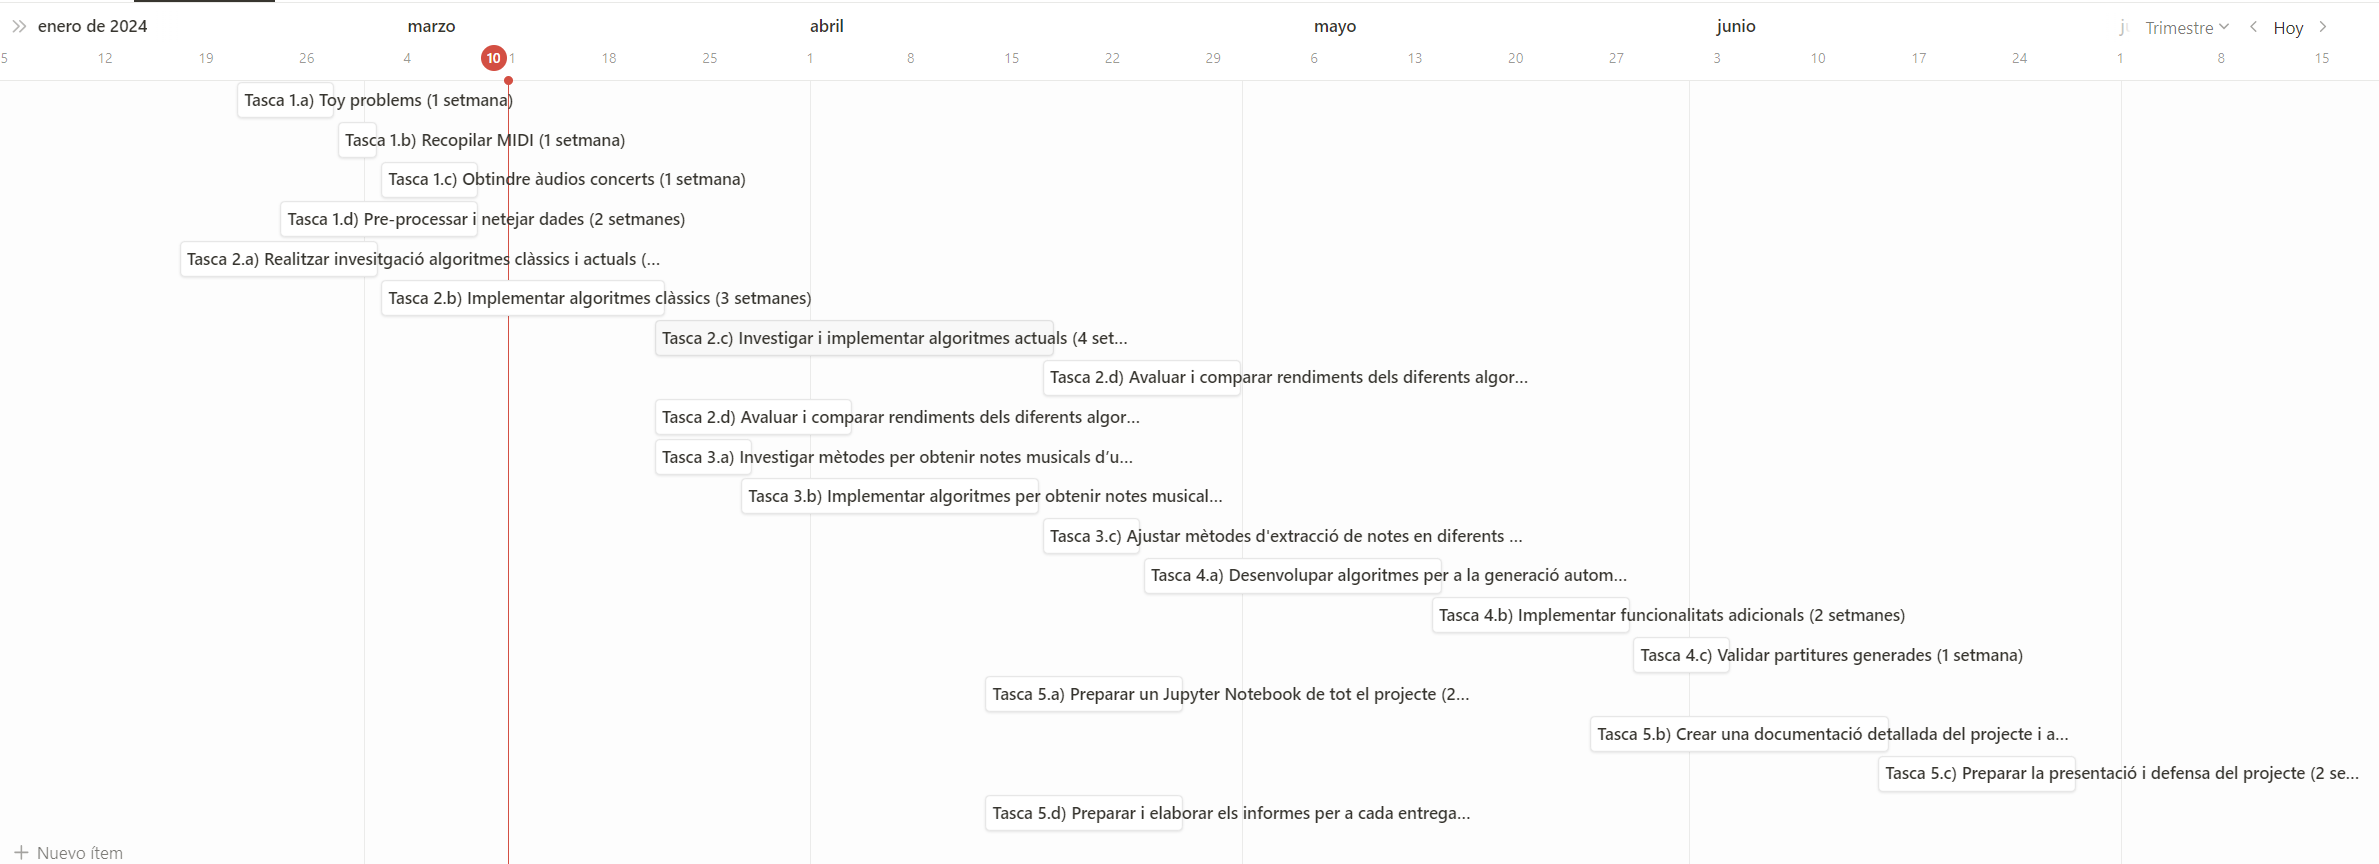
\includegraphics[width=\textwidth]{img/Diagrama de Gantt Claro Fecha.png}
    \caption{Diagrama de Gantt del projecte.}
    \label{fig:gantt}
\end{figure*}

Com es pot observar, les tasques de l'apartat 5 (documentació) són més paral·leles, és a dir, realment s'aniran realitzant durant el desenvolupament del projecte.
En total s'ha aconseguit ajustar en el plaç de temps donat tot i que per a aconseguir-ho s'haurà de realitzar alguna hora extra, sobretot en la part inicial del projecte.

\section{Development}


\section{Conclusions}

.... ..  .... .. .... ... ..... ... ..... ... ... ..... .... .
.... ..  .... .. .... ... ..... ... ..... ... ... ..... .... .
.... ..  .... .. .... ... ..... ... ..... ... ... ..... .... .
.... ..  .... .. .... ... ..... ... ..... ... ... ..... .... .
.... ..  .... .. .... ... ..... ... ..... ... ... ..... .... .
.... ..  .... .. .... ... ..... ... ..... ... ... ..... .... .
.... ..  .... .. .... ... ..... ... ..... ... ... ..... .... .
.... ..  .... .. .... ... ..... ... ..... ... ... ..... .... .
.... ..  .... .. .... ... ..... ... ..... ... ... ..... .... .
.... ..  .... .. .... ... ..... ... ..... ... ... ..... .... .
.... ..  .... .. .... ... ..... ... ..... ... ... ..... .... .
.... ..  .... .. .... ... ..... ... ..... ... ... ..... .... .
.... ..  .... .. .... ... ..... ... ..... ... ... ..... .... .
.... ..  .... .. .... ... ..... ... ..... ... ... ..... .... .

\section*{Agraïments}

... ..  .... .. .... ... ..... ... ..... ... ... ..... .... .
.... ..  .... .. .... ... ..... ... ..... ... ... ..... .... .
.... ..  .... .. .... ... ..... ... ..... ... ... ..... .... .
.... ..  .... .. .... ... ..... ... ..... ... ... ..... .... .
.... ..  .... .. .... ... ..... ... ..... ... ... ..... .... .


\bibliographystyle{plain}
\bibliography{biblio}


\appendix

\section*{Apèndix}

\setcounter{section}{1}

\subsection{Secció d'Apèndix}


... ..  .... .. .... ... ..... ... ..... ... ... ..... .... .
.... ..  .... .. .... ... ..... ... ..... ... ... ..... .... .
.... ..  .... .. .... ... ..... ... ..... ... ... ..... .... .
.... ..  .... .. .... ... ..... ... ..... ... ... ..... .... .
.... ..  .... .. .... ... ..... ... ..... ... ... ..... .... .

\subsection{Secció d'Apèndix}


... ..  .... .. .... ... ..... ... ..... ... ... ..... .... .
.... ..  .... .. .... ... ..... ... ..... ... ... ..... .... .
.... ..  .... .. .... ... ..... ... ..... ... ... ..... .... .
.... ..  .... .. .... ... ..... ... ..... ... ... ..... .... .
.... ..  .... .. .... ... ..... ... ..... ... ... ..... .... .


\end{document}

